\section{SAPHSOLVE Post-Processing Engine Development}
\label{sec:saphsolve-devel}

Accident sequence \acrshort{mcs} generated during \acrshort{pra} often require manipulation to address specific modeling concerns, such as post-accident scenarios, \acrshort{ccf} modeling, and the elimination of mutually exclusive events. Rather than re-quantify the entire model for each manipulation---a process that can be computationally expensive---the post-processing engine in \acrshort{saphire} allows users to manipulate generated \acrshort{mcs} by defining rules.

The initial implementation of \acrshort{mcs} manipulation in \acrshort{saphire} dates back to 1996 and was known as the recovery engine \cite{Smith1996SAPHIRE}. To utilize the post-processing engine, users create a \emph{Rule File} through the \acrshort{gui}. This file consists of a series of \texttt{if}-\texttt{else} statements that specify the events or conditions under which certain actions are performed. Depending on the conditions defined by the user in the Rule File, the \acrshort{saphire} post-processing engine updates the generated \acrshort{mcs} and their associated failure probabilities for each accident sequence.

Although the current post-processing engine integrates seamlessly with other engines in the \acrshort{saphire} \acrshort{api} and functions effectively, the \acrshort{saphire} team prioritizes maintainability. Given the rapid evolution of computational resources, programming languages, and software environments, the team commits to adopting newer technologies to ensure long-term functionality of \acrshort{saphire}, its \acrfull{spar} models, and related components. For a more comprehensive description of Rule Files, including keywords and examples, see the \acrshort{saphire} Manual Volume~3 \cite{saphire_manual}.

\subsection{Core Functions of the New Post-Processing Engine}
\label{sec:core-functions}

The new post-processing engine has been completely re-built from the ground up and comprises five core functions. Figure~\ref{fig:postproc-engine-schematic} provides a simple schematic of how the post-processing engine interacts with input files, rules, and the resulting updated output. Table~\ref{tab:coreFunctions} summarizes the five core components of the new post-processing engine and their primary roles. 

\usetikzlibrary{positioning,arrows.meta}
\begin{figure}[h]
  \centering
  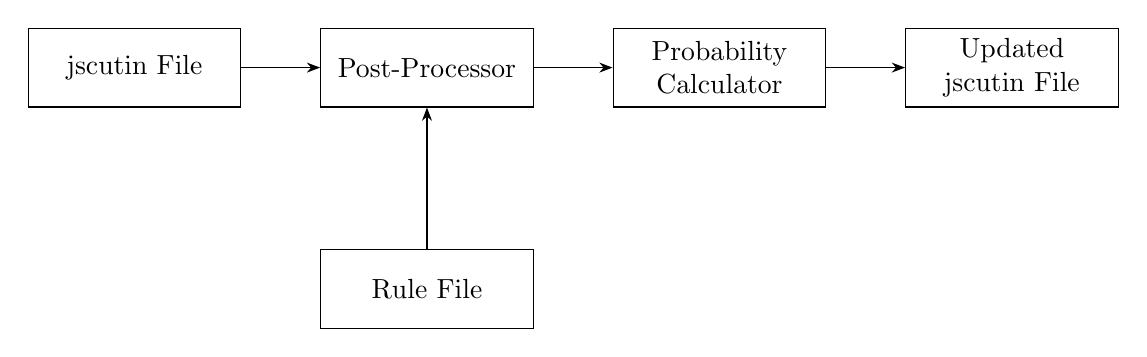
\begin{tikzpicture}[
      >=Stealth,                   % arrow tip
      every node/.style = {draw, rectangle,
                           minimum width = 2.7cm,
                           minimum height = 1cm,
                           align = center}
    ]
    % Nodes
    \node (jscutin)            {\acrshort{jscutin} File};
    \node[right=of jscutin]    (engine) {Post-Processor};
    \node[below=1.8cm of engine] (rulefile) {Rule File};
    \node[right=of engine]     (calc)   {Probability\\Calculator};
    \node[right=of calc]       (updated){Updated\\\acrshort{jscutin} File};

    % Arrows
    \draw[->] (jscutin) -- (engine);
    \draw[->] (engine)  -- (calc);
    \draw[->] (calc)    -- (updated);
    \draw[->] (rulefile)-- (engine);
  \end{tikzpicture}
  \caption{Post-processing engine: schematic representation.}
  \label{fig:postproc-engine-schematic}
\end{figure}

\begin{table}[h]
\centering 
\caption{Core functions of the new post-processing engine in \acrshort{saphire}.}
\begin{tabular}{@{}ll@{}}
\toprule
\textbf{Function}                  & \textbf{Description}                                                                                             \\ 
\midrule
\acrshort{jscutin} Parser                & Parses the \acrshort{jscutin} file containing \acrshort{mcs} and \acrlong{be}.                                  \\
Rule File Parser                   & Reads user-defined rules; converts them to \acrshort{json}.                              \\
Post-Processor                     & Applies Rule File logic to parsed \acrshort{jscutin}, filtering or modifying the \acrshort{mcs}.                   \\
Probability Calculator             & Re-calculates sequence failure probabilities based on the updated \acrshort{mcs}.                                     \\
\acrshort{jscutin} Writer                     & Outputs the final \acrshort{jscutin} file with revised probabilities and \acrshort{mcs}.                                \\ 
\bottomrule
\end{tabular}
\label{tab:coreFunctions}
\end{table}

The \acrshort{jscutin} file and the rule file are used as inputs to the post-processing engine. A typical Rule File contains statements and actions, often expressed in a simple symbolic syntax. For instance:
\begin{itemize}
    \item The symbol ``\texttt{|}'' can be used to comment out lines.
    \item The symbol ``\texttt{*}'' indicates an \emph{AND} operation.
    \item The symbol ``\texttt{+}'' indicates an \emph{OR} operation.
\end{itemize}
The \acrshort{jscutin} file is a \acrshort{json}-based file containing \acrshort{saphsolve} engine quantification results and \acrlong{be} information. As discussed previously, users may wish to update existing quantification results without re-quantifying the entire \acrshort{pra} model. To do so, a rule file is created to specify updates to the \acrshort{mcs}. The post-processing engine parses both the \acrshort{jscutin} file and the rule file, executes the specified actions, modifies the \acrshort{mcs} list accordingly, recalculates the \acrshort{mcs} probability using the \acrshort{mcub} approach, and ultimately outputs a new \acrshort{jscutin} file. The following files from the generic \acrshort{pwr} model \cite{Aras2024Generic} are provided in the appendices to offer further insights:

\begin{itemize}
\item The abbreviated ACC \acrshort{jscutin} file is presented in Section11.4, containing only the necessary details.
\item The post-processed ACC \acrshort{jscutin} file is included in Section11.5.
\item The rule file can be found in Section11.6.
\item The proposed rule file \acrshort{json} schema is included in Section11.7.
\item The parsed and \acrshort{json}-formatted generic \acrshort{pwr} rule file is available in Section~11.8.
\end{itemize}

The post-processing engine is implemented in C\#. The \acrshort{jscutin} file or rule file can be directly supplied to the engine, or the engine can retrieve input files from a database if required. Converting the rule file into a \acrshort{json} format improves portability and offers efficient communication channels with other engines or databases. During this conversion, the original rule file contents are transformed into two lists: the \emph{condition list} and the \emph{action list}. In a typical rule file (such as the example in Section~11.6), users define conditional statements that specify actions to be taken for basic events within the generated \acrshort{mcs}. The action list encompasses potential adjustments or filtering steps, retaining all desired possibilities in \acrshort{json} objects.

\subsubsection{Masked Basic Event Number Allocation}
\label{sec:masked-event-allocation}

The rule file contains assigned basic event names, whereas the \acrshort{jscutin} file includes \acrshort{mcs} that are masked. The post-processing engine can \emph{unmask} the \acrshort{mcs} information during processing and then \emph{re-mask} it when generating the updated \acrshort{jscutin} file. This masking technique enables faster manipulation of large data sets.

\begin{itemize}
    \item \textbf{Bits 0--17:} Event number
    \item \textbf{Bits 18--24:} Phase information
    \item \textbf{Bits 25--29:} Model type
    \item \textbf{Bit 30:} Basic event tag
    \item \textbf{Bit 31:} Complement information
\end{itemize}

\noindent Figure~\ref{fig:bit-dist-masked} shows how these 32 bits are allocated in the masked identifier. As a simple example, consider an event, encoded as the integer value \(\displaystyle 33816579\). When parsed, this corresponds to: \[
\text{Event ID} = 3, \quad
\text{Phase} = 1, \quad
\text{Model Type} = 1.
\]

\begin{figure}[htbp]
  \centering
    % -----------------------------------------------------------------
    % New, light 5-colour pastel palette
    % (RGB values taken from ColorBrewer, Pastel-1)
    % -----------------------------------------------------------------
    \definecolor{pComplement}{RGB}{251,180,174}   % pastel-red
    \definecolor{pBasicEvt} {RGB}{179,205,227}   % pastel-blue
    \definecolor{pModel}    {RGB}{204,235,197}   % pastel-green
    \definecolor{pPhase}    {RGB}{222,203,228}   % pastel-purple
    \definecolor{pEvtNum}   {RGB}{254,217,166}   % pastel-orange

    % ---------------------------------------------------------------
    % Convenience macro for rotated field labels (unchanged)
    % ---------------------------------------------------------------
    \newcommand{\bitlabel}[2]{%
      \bitbox[]{#1}{% 
        \raisebox{0pt}[4ex][0pt]{%
          \turnbox{45}{\fontsize{8}{16}\selectfont#2}%
        }%
      }%
    }


    % ---------------------------------------------------------------
    % Bit-field diagram
    % ---------------------------------------------------------------
    \begin{bytefield}[endianness=big,
                      bitwidth=14pt,
                      bitheight=\widthof{~BE~},
                      boxformatting={\centering\small}]{32}
    
      % Row with field names
      \bitlabel{1}{Complement} &
      \bitlabel{1}{Basic Event Tag} \\
    
      \bitheader{0-31} \\
    
      % Row with symbolic field identifiers
      \bitbox{1}[bgcolor=pComplement]{\rotatebox{90}{C}} &
      \bitbox{1}[bgcolor=pBasicEvt]{\rotatebox{90}{BE}} &
      \bitbox{5}[bgcolor=pModel]{MODEL TYPE} &
      \bitbox{7}[bgcolor=pPhase]{PHASE} &
      \bitbox{18}[bgcolor=pEvtNum]{EVENT IDENTIFIER} \\[1.2ex]
    
      % Row with an example 32-bit value
      \bitheader{0-31} \\
    
      \bitbox{1}[bgcolor=pComplement]{0} &
      \bitbox{1}[bgcolor=pBasicEvt]{0} &
      \bitboxes*{1}[bgcolor=pModel]{00001} &
      \bitboxes*{1}[bgcolor=pPhase]{0000001} &
      \bitboxes*{1}[bgcolor=pEvtNum]{000000000000000011}
    
    \end{bytefield}
  \caption{Bitwise Encoding Scheme for Mapping Event Information to a 32-bit Word.}
  \label{fig:bit-dist-masked}
\end{figure}